\documentclass[t,handout]{beamer}   % overlays

\usetheme{Madrid}
\usecolortheme{beaver}
\usepackage{tikz}
\usetikzlibrary{fit,arrows,calc,positioning}

%\usepackage{emerald} 
\usepackage[T1]{fontenc} 


\usepackage{graphicx}
\usepackage{epsfig}
\usepackage{psfrag}
\usepackage[english]{babel}
\usepackage{listings}
\usepackage{courier}
\usepackage{color}
\usepackage[backend=bibtex,style=ieee]{biblatex}

\lstset{
	language=Ruby,
	basicstyle=\footnotesize\ttfamily\color{black},
	commentstyle = \footnotesize\ttfamily\color{red},
	keywordstyle=\footnotesize\ttfamily\color{blue},
	stringstyle=\footnotesize\ttfamily\color{black},
%	columns=fixed,
%	numbers=left,    
	numberstyle=\tiny,
	stepnumber=1,
	numbersep=5pt,
	tabsize=1,
	extendedchars=true,
	breaklines=true,            
	frame=b,         
	showspaces=false,
	showtabs=true,
	xleftmargin=6pt,
	framexleftmargin=6pt,
	framexrightmargin=2pt,
	framexbottommargin=4pt,
	showstringspaces=false      
}

\lstloadlanguages{
         Ruby,HTML
}

\graphicspath{ {./images/} }  % Figures path - used in graphicx

%\selectcolormodel{cmyk}

\mode<presentation>

\renewcommand*{\bibfont}{\tiny}

\newcommand{\dred}{darkred!90!black}
\newcommand{\written}{\ECFJD\textcolor{cyan!50!white}}
\newcommand{\hlight}{\textcolor{\dred}}
\newcommand{\Ex}{\textcolor{\dred}{Ex. }}

% remove navigation symbols in full screen mode
\setbeamertemplate{navigation symbols}{}  
\setbeamertemplate{blocks}[rounded][shadow=false]
\setbeamertemplate{itemize items}[default]
\setbeamertemplate{enumerate items}[default]
\setbeamertemplate{sections/subsections in toc}[circle]
\setbeamercolor{note page}{fg=black}

\setbeamercolor{title}{fg=\dred}
\setbeamercolor{frametitle}{fg=white}
\setbeamercolor{frametitle}{bg=\dred}
\setbeamercolor{structure}{fg=black,bg=white}
\setbeamercolor{background canvas}{bg=white,fg=black}
\setbeamercolor{normal text}{fg=black,bg=white}
\setbeamercolor{item}{fg=red!80!black,bg=white!}
\addtobeamertemplate{block begin}{\setbeamercolor{block title}{fg=white,bg=\dred}
\setbeamercolor{block body}{fg=\dyellow,bg=gray!50!black}}{}



\addbibresource{bib/aws.bib}

\title[FERPA, UNM, and AWS]
{FERPA, UNM, and AWS}

\author[Heileman] % (optional, use only with lots of authors)
{\bf Gregory L. Heileman}

\institute[]
{Informatics Laboratory \\
Department of Electrical \& Computer Engineering \\
University of New Mexico}

\date[June 26, 2015]

\begin{document}

\begin{frame}
  \titlepage
\end{frame}
\note{Talk for 10 minutes} 

\addtobeamertemplate{frametitle}{}{%
\begin{tikzpicture}[remember picture,overlay]
\node[anchor=north east,yshift=-1pt] at (current page.north east) {
\includegraphics[width = 1in]{UNMLogo.png}};
\end{tikzpicture}}

%%%%%%%%%%%%%%%%%%%%%%%%%%%%%%%%%%%%%%%%%%%%%%%%%%%%%%

%\section*{Outline}
%
%\begin{frame}  \frametitle{Outline}  
%	\tableofcontents
%\end{frame}

\section{Introduction}

\begin{frame}{Why are we here?}
\textbf{We are moving aggregated student data to Amazon for cohort analysis.}
\\~\\
{\small This is happening now --- but we need help to do it right.}
\\~\\
\pause
We are a lab with research experience in data analytics, cyber-security\footnote{Recent graduations has this concentrated in a couple of us.}, and cloud computing experience. We are not a disciplined devops shop:
\pause
{\small
\begin{itemize}
\item We do not have permanent staff\footnote{Well, some of our PhD students seem pretty close to permanent.}
\pause
\item We do not have 24-hour response.
\pause
\item We do not have operational cyber-security experience.
\end{itemize}
}
\end{frame}

\begin{frame}{Security Profile \& Controls}
\textbf{FIPS 199, 200 and NIST SP800-53}
{\small
\begin{itemize}
\item FIPS helps you decide how important your data is
\item NIST helps you select the controls to protect it
\end{itemize}
}

\textbf{Other Universities}
{\small
\begin{itemize}
\item UNC Asheville, Carnegie Mellon University rate student data at high
\item Colorado University, Loyola University rate student data at moderate
\end{itemize}
}
~\\~\\
High implies loss-of-life; we selected moderate as our guideline for security control selection from NIST SP800-53~\footnote{Moderate doesn't mean insignificant. The number of required controls at the moderate level is still daunting, much larger than low, and slightly less than high.}.


\end{frame}

\section{Technical Components}

\begin{frame}{Technical Components}
	\begin{center}
		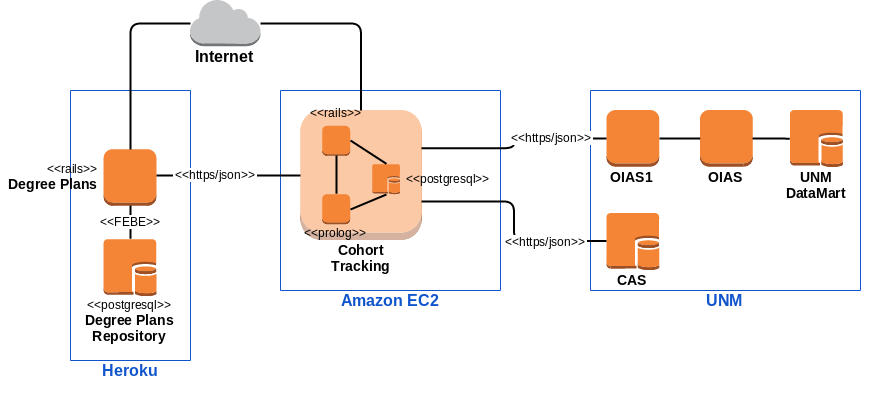
\includegraphics[width=\textwidth]{technical_architecture.png}
	\end{center}
\end{frame}


\section{Responsibilities}

\begin{frame}{Responsibilities - Infrastructure}
 	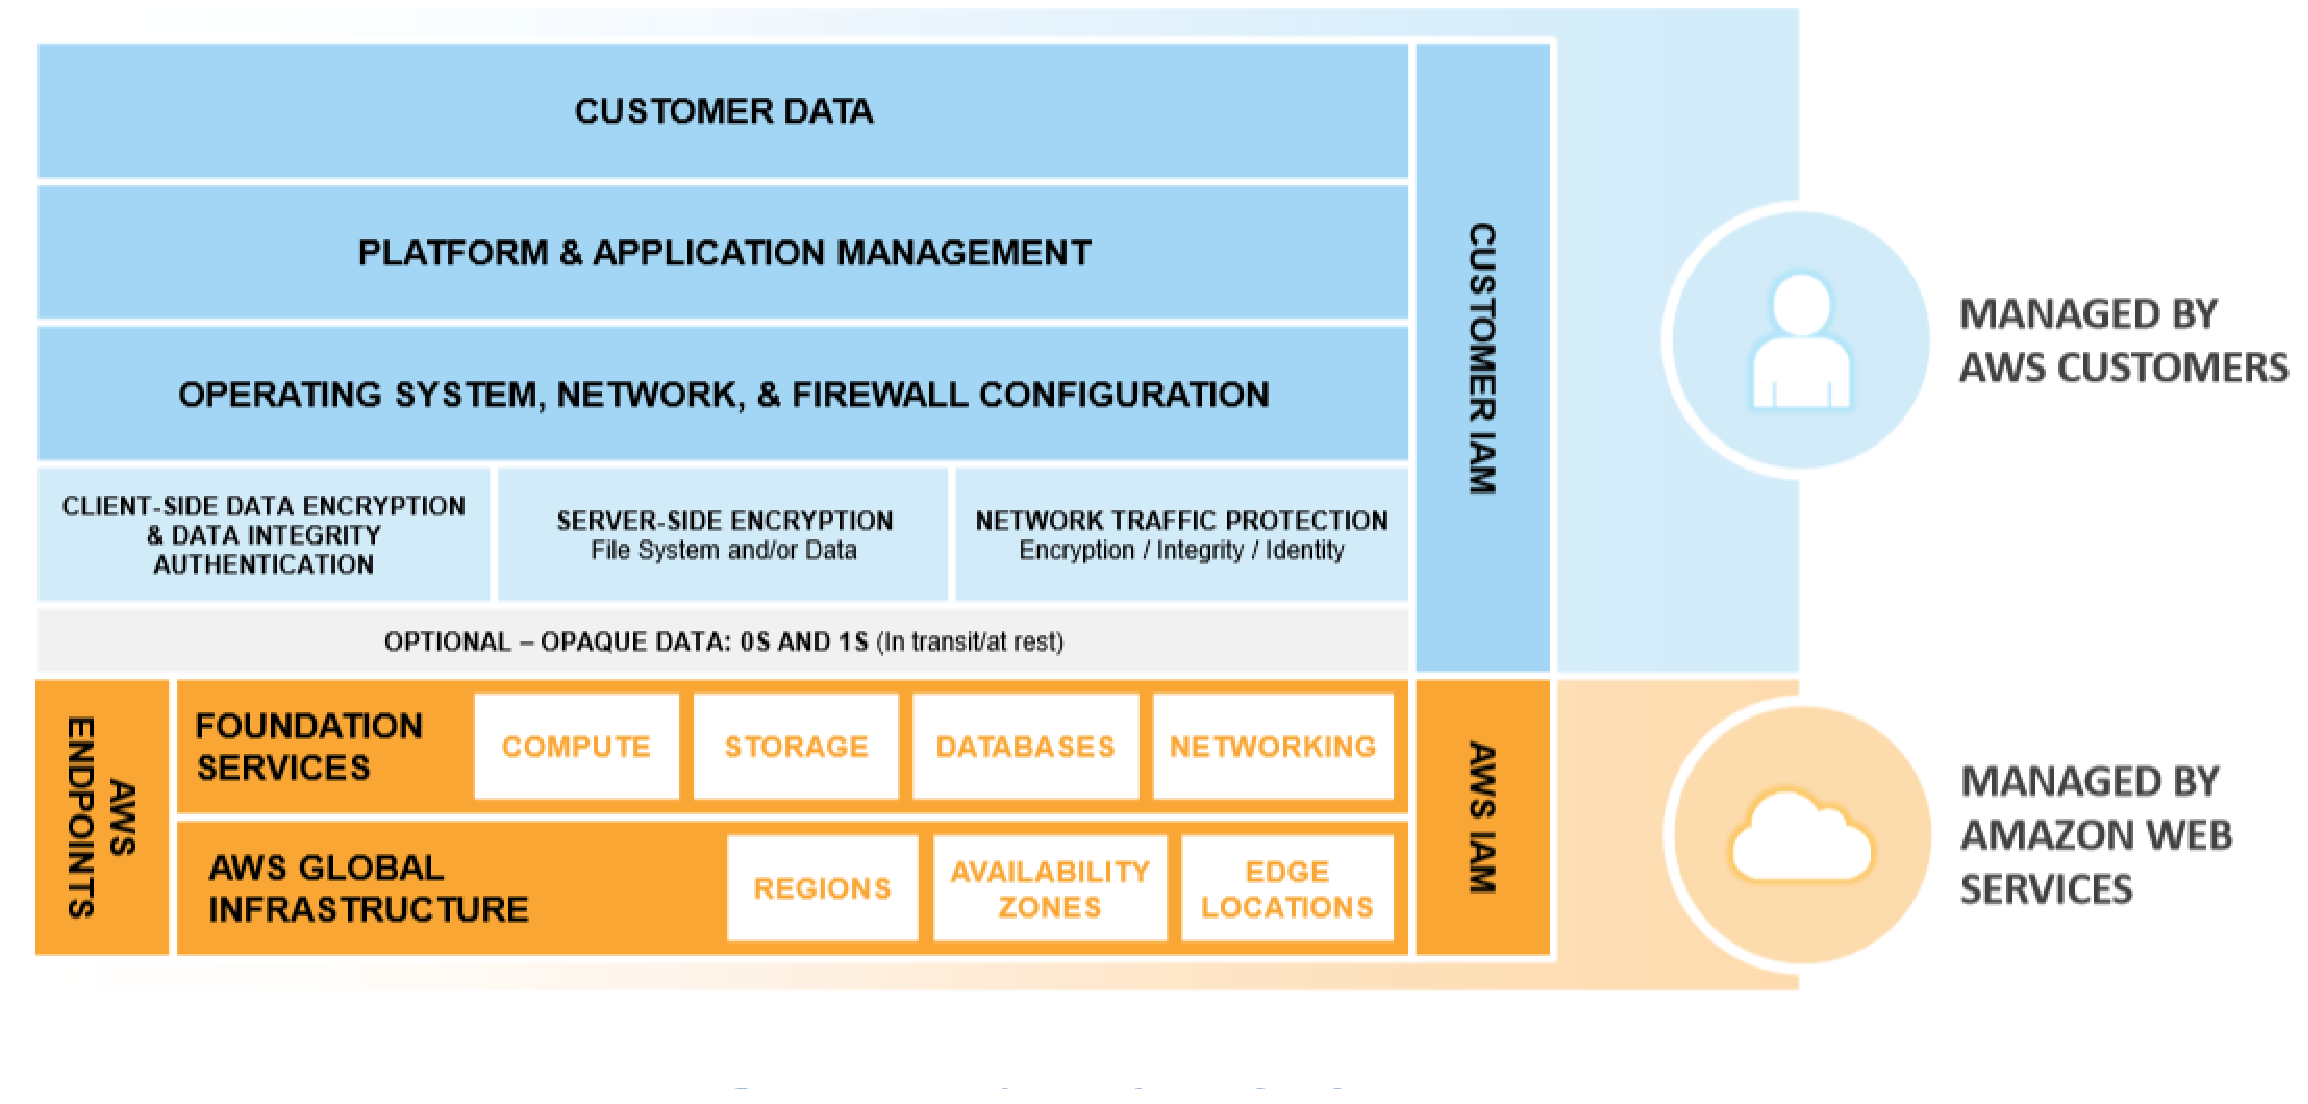
\includegraphics[width=\textwidth]{442-mod.pdf} \\
 	{\tiny Extracted from content provided by Amazon Web Services~\footfullcite{Aws:15}.}
\end{frame}

\begin{frame}{Responsibilities - Containers}
 	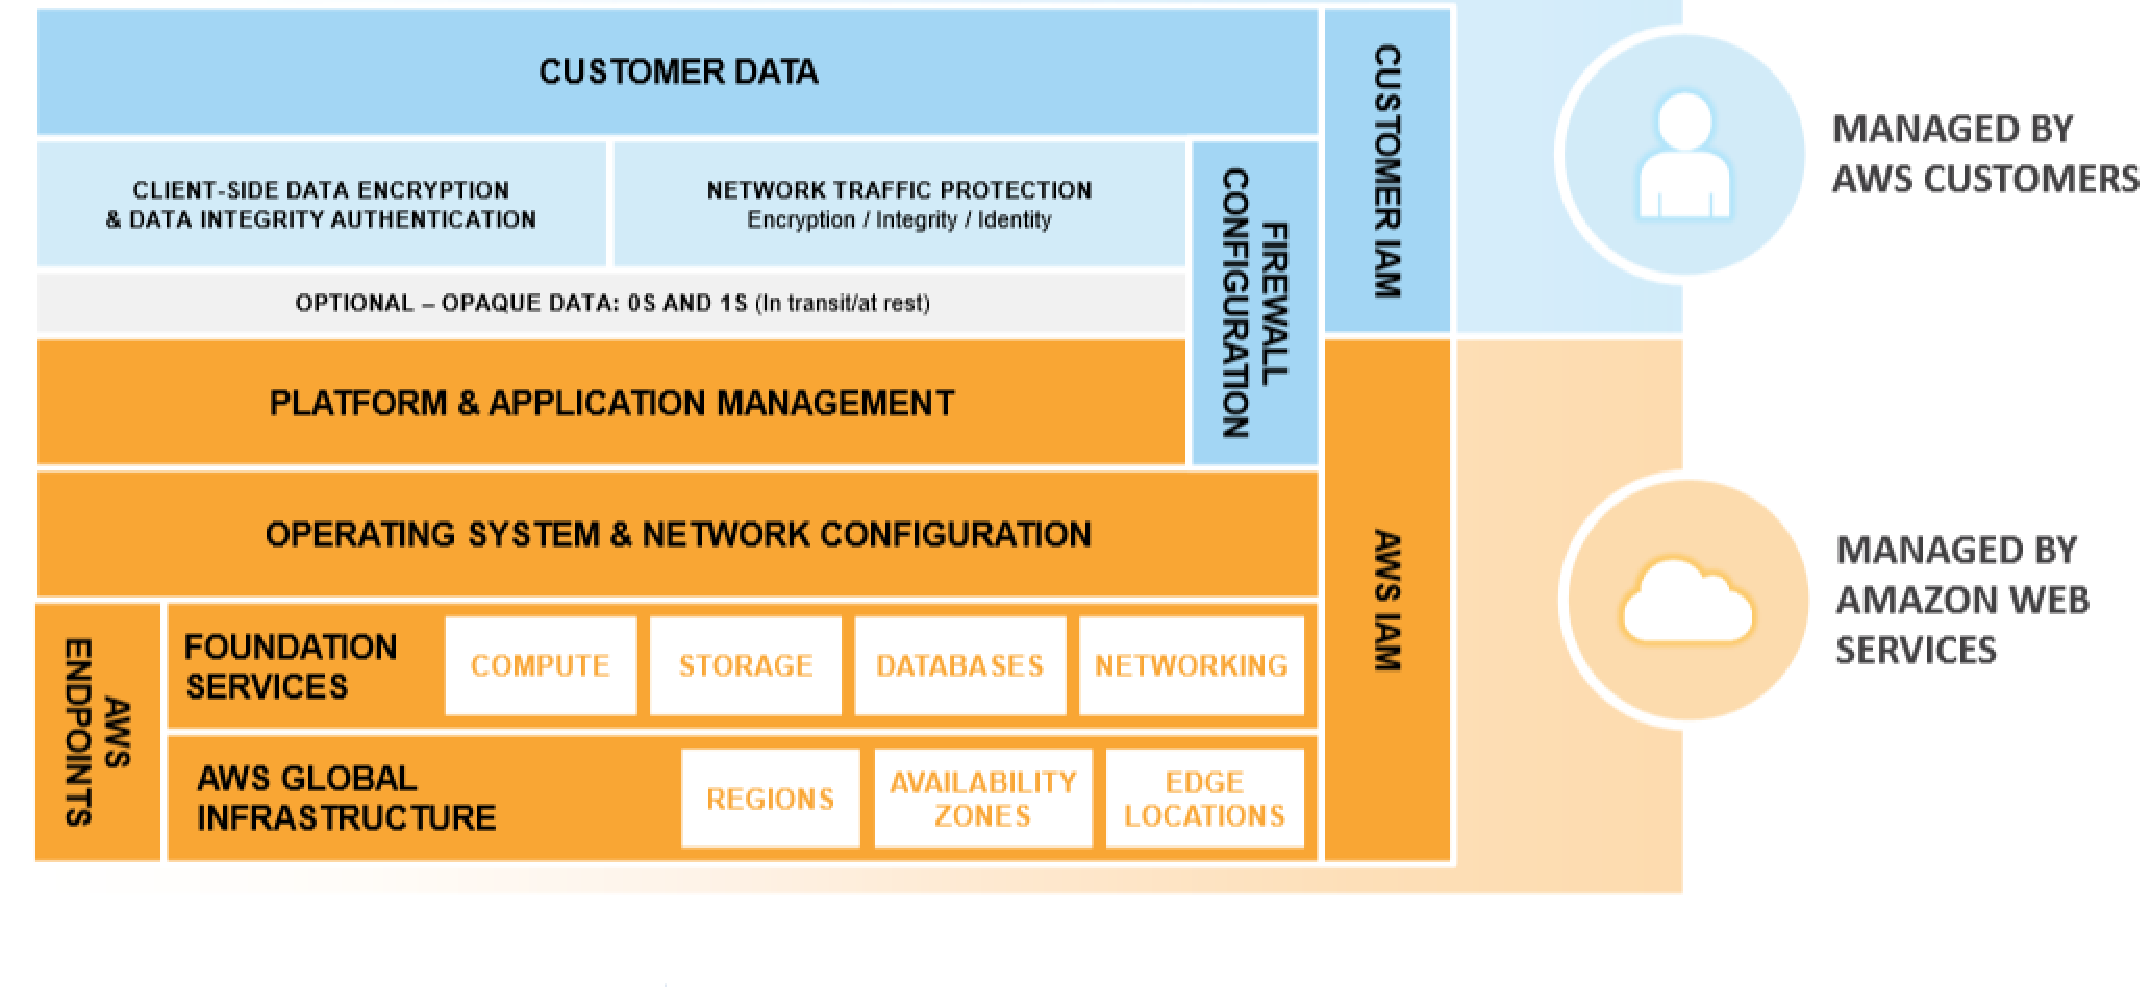
\includegraphics[width=\textwidth]{445-mod.pdf}
\end{frame}

\begin{frame}{Responsibilities - Abstract Services}
 	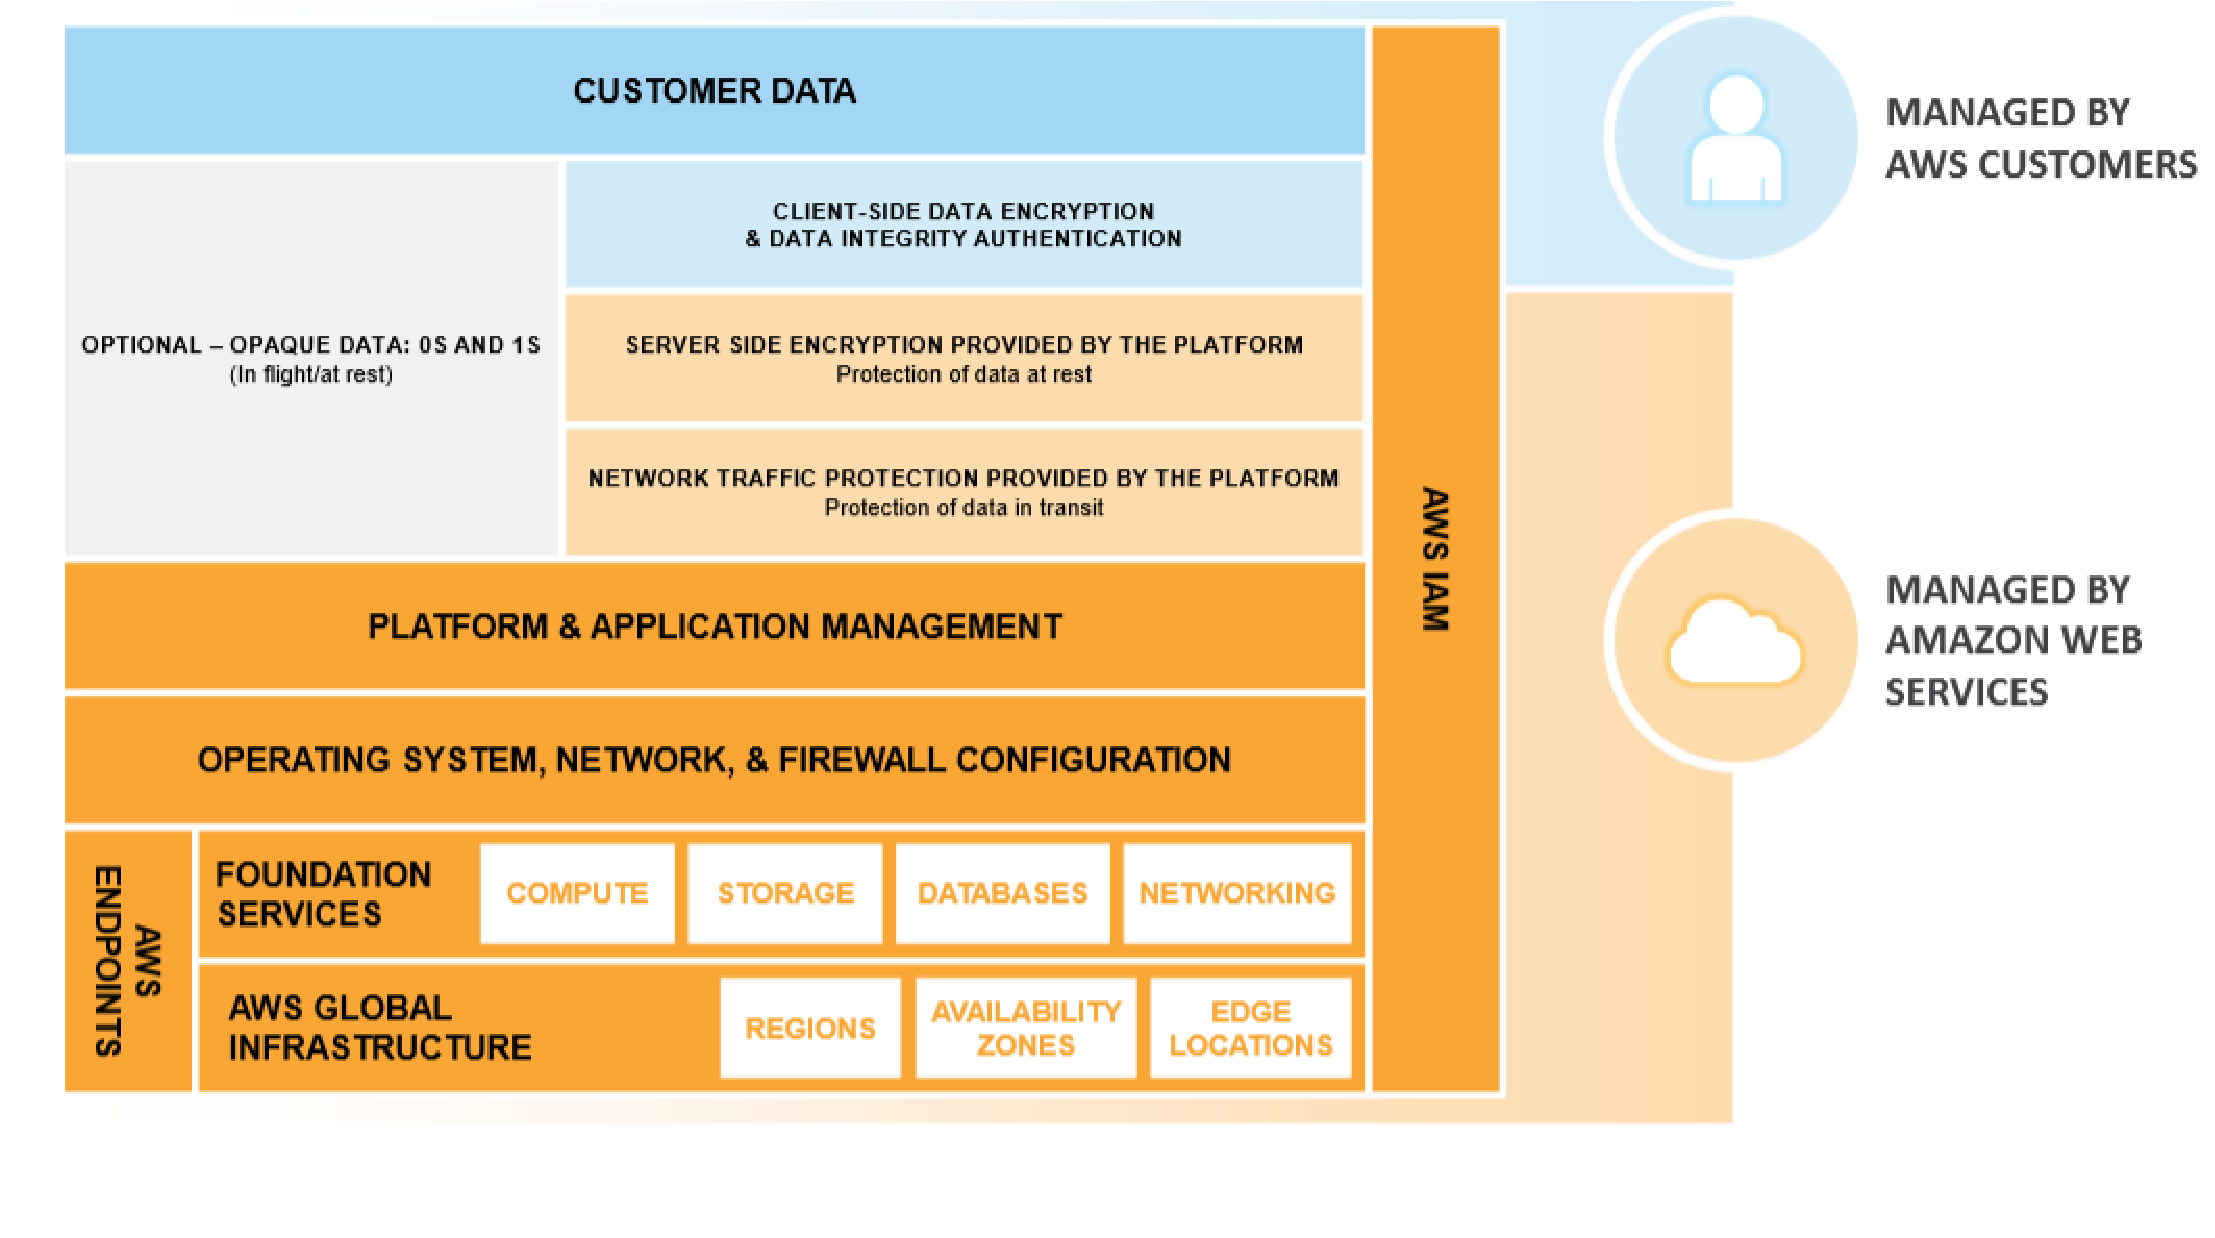
\includegraphics[width=\textwidth]{448-mod.pdf}
\end{frame}

\begin{frame}{Our Responsibilities - Heroku}

\textbf{Heroku is a PaaS Offering}
{\small
\begin{itemize}
\item We \textbf{don't} maintain the Rails or PostreSQL installation
\item We \textbf{do} maintain the running application
\begin{itemize}
\item This application does not serve PII
\item It only handles non-confidential degree plan data
\end{itemize}
\end{itemize}
}
\centering
\textbf{We communicate via HTTPS and sanitize data from this system}

\end{frame}

\begin{frame}{Our Responsibilities - AWS}

\textbf{OS, Network, FW Configuration}
{\small
\begin{itemize}
\item Elastic Compute Cloud (EC2) VMs run SELinux/Redhat, UFW
\item We don't manage UNM VMs or Firewalls
\item We manage host firewalls only, and we don't maintain a VPC (for now)
\end{itemize}
}

\pause

\textbf{Platform \& Application Management}
{\small
\begin{itemize}
\item Ruby/Rails --- Runs on EC2; manually patched when required via the \textit{bundler} and \textit{gem} utilities
\item Redis --- Currently migrating to Amazon RDS and Elasticache
\item Prolog --- Patched via operating system utilities
\end{itemize}
}

\pause

\textbf{Student Data}
{\small
\begin{itemize}
\item Data is encrypted at rest~\footfullcite{BeHo:14} and in motion (HTTPS or equivalent)
\end{itemize}
}

\end{frame}

\begin{frame}{Identity Management, Accounts, and Keys}

\textbf{UNM and Local Identity Management}
{\small
\begin{itemize}
\item Local accounts on EC2 and amazon are managed using UNM password policies (strong passwords with six month rotation)
\item Application access is authorized via local whitelists and CAS authentication to UNM
\item We only allow administrative access via sudo
\item We use Amazon IAM as much as possible
\end{itemize}
}

\textbf{Amazon Identity Management}
{\small
\begin{itemize}
\item Phasing out SSH access to running systems
\item Migrating to multi-factor authentication (e.g. Google Authenticator)~\footfullcite{MFA:15}
\item Amazon key management for key storage
\end{itemize}
}
\end{frame}

\begin{frame}{Security Monitoring}

\textbf{CloudWatch}
{\small
\begin{itemize}
\item Syslog, performance, communication, etc.
\item Early indicator that VMs have been compromised
\begin{itemize}
\item Higher usage
\item New VM creation
\item Very large instance creation (great for mining bitcoin, for example)
\end{itemize}
\end{itemize}
}

\textbf{CloudTrail}
{\small
\begin{itemize}
\item Compliance monitoring, user activity tracking, API access
\item Good for initial intrusion detection
\begin{itemize}
\item New API access
\item Excessive API access
\end{itemize}
\end{itemize}
}
~\\

\centering
\textbf{We don't monitor these as well as we should.}

\end{frame}

\begin{frame}{Wrapping Up}

\textbf{We have some things in process...}
{\small
\begin{itemize}
\item NIST SP800-53 mappings and documentation
\item Migration to VPC
\item More automation
\end{itemize}
}

\textbf{...we are doing some things well...}
{\small
\begin{itemize}
\item Controlled VM images
\item Authentication integration
\item At rest/in motion encryption
\item Patching
\end{itemize}
}

\textbf{...but we need some help.}
{\small
\begin{itemize}
\item Monitoring, management, continuity
\item Security auditing in all phases
\end{itemize}
}

\end{frame}

%\begin{frame}{Bibliography}
% 	\def\newblock{}	
%	\printbibliography
%\end{frame}

\end{document}
